\documentclass{standalone}
\usepackage{../../../../preamble_formulas}

% Define arrow's style
\usetikzlibrary{decorations.markings}
 
% Arrow style
\tikzset{decorated arrows/.style={
    postaction={
        decorate,
        decoration={
            markings,
            mark=between positions 0 and 1 step 15mm with {\arrow[black]{stealth};}
            }
        },
    }
}
 
 
\begin{document}
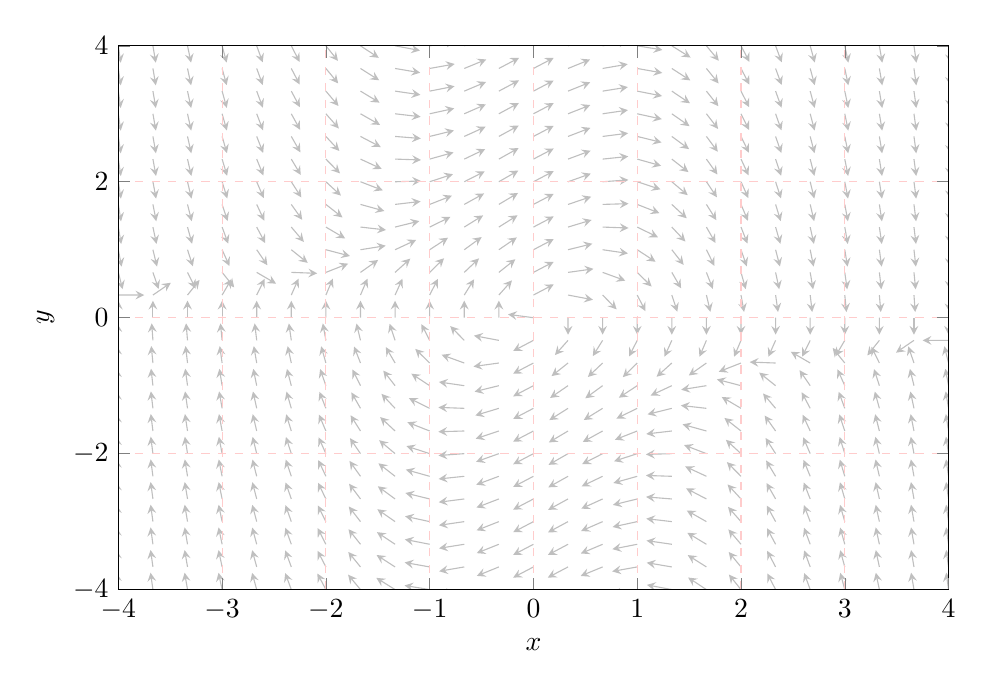
\begin{tikzpicture}

  \begin{axis}[
      grid=both,
      grid style={dashed,red!20},
      xmin = -4, xmax = 4,
      ymin = -4, ymax = 4,
      width = \textwidth,
      height = 0.7\textwidth,
      xlabel = {$x$},
      ylabel = {$y$},
      title={},
      view = {0}{90},
    ]

    % Vector Field
    \addplot3[
      quiver = {
          u = {y/sqrt(y^2+(0.8*(1-x^2)*y-x)^2)},
          v = {(0.8*(1-x^2)*y-x)/sqrt(y^2+(0.8*(1-x^2)*y-x)^2)},
          scale arrows = 0.25,
        },
      -stealth,
      domain = -4:4,
      domain y = -4:4,
      lightgray]
    {0};

  \end{axis}
\end{tikzpicture}

\end{document}